\subsection{Other Circuits:}

The circuits shown in figures 3.4.0 and 3.4.1 are very similar, both use a {\bfseries\itshape Square} signal at a 0.5 $H_{z}$ frequency that comes from the output of the {\itshape functions generator}, which it's connected to a resistor $R_{B}$ that is in series whit the {\bfseries\itshape Base} terminal. The difference lays in the {\bfseries\itshape NPN} transistor to which they are connected.

\begin{multicols}{2}
\begin{figure}[H]
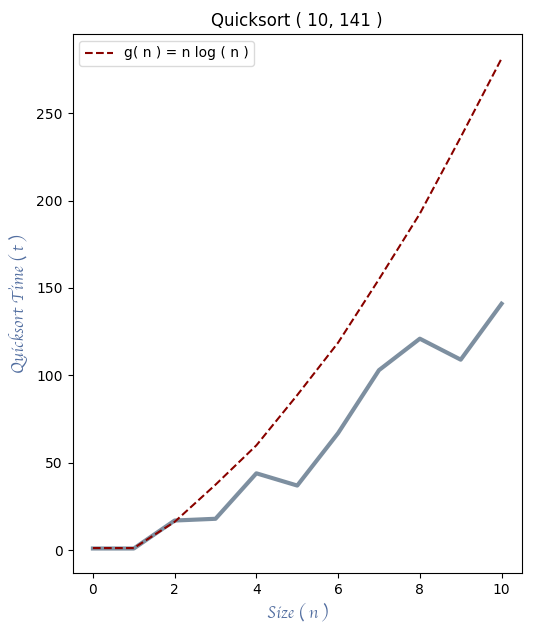
\includegraphics[scale=.68]{p3.png}
\centering \linebreak \linebreak Figure 3.4.0:  2N2222A - LED circuit.
\end{figure}

\begin{figure}[H]
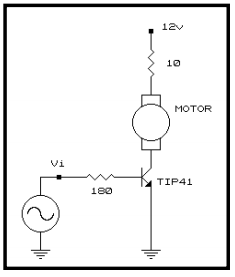
\includegraphics[scale=.605]{p4.png}
\centering \linebreak \linebreak Figure 3.4.1: TIP41 - Motor circuit.
\end{figure}
\end{multicols}

\begin{itemize}
\item For the circuit of Figure 3.4.0, as we mention, we connect in series a {\itshape Square} signal at 0.5 $H_{z}$ and the resistor $R_{B} = 1K \Omega$. In $R_{C}$, we use a resistor of 100 $\Omega$ at 25w and the transistor used it's a {\bfseries\itshape 2N2222A}. As we can see in Figure 3.4.0, the LED its connected implicitly to the 12 V source, such that, it will be "turned on". But, when the {\itshape Square} signal its on the "positive" region, it means that the {\bfseries Base} terminal it receiving voltage and current, in consequence, the LED will be {\itshape brighter} until the positive cycle finishes. \hfill \break

\item For the circuit of Figure 3.4.1, same as Figure 3.4.0, we connect in series a {\itshape Square} signal at 0.5 $H_{z}$ and the resistor $R_{B} = 180 \Omega$. In $R_{C}$, we use a resistor of 10 $\Omega$ at 25w and the transistor used it's a {\bfseries\itshape TIP41}, this is a power transistor, and the use is identical to the normal transistors, having as special characteristics the high voltages and currents that they have to support and, therefore, the high powers to be dissipated. As we can see in Figure 3.4.1, the Motor its connected implicitly to the 12 V source, but, even that it's receiving voltage and current, this is insufficient to "turn on" the device. But, when the {\itshape Square} signal its on the "positive" region the "energy" that the device receives it's enough to turn it on until the positive cycle finish. This because the transistor on {\bfseries\itshape Common - Emitter} configuration increase current and voltage.
\end{itemize}

\pagebreak